\documentclass{article}

\usepackage{algorithmic}
\usepackage{amsmath}
\usepackage{graphicx}
\usepackage{hyperref}
\usepackage{booktabs}
\usepackage{verbatim}

\begin{document}

\title{Final Exam}
\author{Geoffrey Ulman\\
        CSI873}
\date{December 2011}
\maketitle

\section{Model}\label{Model}

The support vector machine constrained polynomial optimization problem was modeled and solved using AMPL (\url{www.ampl.com/}). Computations were performed using the LOQO solver (\url{www.princeton.edu/~rvdb/loqo/LOQO.html}) on the NEOS server (\url{www.neos-server.org/neos/solvers/}). Once the solution to the dual problem was obtained, the \(\alpha\) values were imported into Java to make the final classification.

Java (version 1.6.0\_27) was used to implement the neural network and training algorithm. The code is available as a Subversion repository on Google Code at \url{http://code.google.com/p/csi873/}. Compiling and running the code requires the Java build tool Maven (\url{http://maven.apache.org/}).

\hline

\begin{verbatim}

model;

# number of training examples
param l;

# number of input parameters (pixels in digit image)
param n;

# weight on xi penalty coefficient in primal problem
param C;

# parameters for polynomial machine kernel
param alpha;
param beta;
param delta;

# output vector (1 or -1)
param y { 1..l };

# input data
param x { 1..l, 1..n };

# dual problem variables and simple constraints
var a {1..l} >= 0, <= C;

maximize obj: sum { i in 1..l } a[i] - 0.5 *
              sum { i in 1..l, j in 1..l } a[i] * a[j] * y[i] * y[j] *
              ( alpha * ( sum { k in 1..n } x[i,k] * x[j,k] ) + beta ) ^ delta;

s.t. const: sum { i in 1..l } a[i] * y[i] = 0;

option solver loqo;

\end{verbatim}

\hline

\section{Two Digit Results}\label{Results2}



\begin{table}
\caption{Digit 2 vs 5 Error}
\begin{center}
\begin{tabular}{llcc}
\toprule
Data Set & Error & \multicolumn{2}{c}{95\% Confidence Interval} \\
\cmidrule(r){3-4}
& & Lower Bound & Upper Bound \\
\midrule
Polynomial Training & 0.000 & 0.000 & 0.000 \\
Polynomial Testing & 0.098 & 0.033 & 0.162 \\
Radial Training & 0.027 & 0.004 & 0.050 \\
Radial Testing & 0.110 & 0.042 & 0.177 \\
\bottomrule
\end{tabular}
\label{error1}
\end{center}
\end{table}

\begin{table}
\caption{All Digits Error}
\begin{center}
\begin{tabular}{llcc}
\toprule
Data Set & Error & \multicolumn{2}{c}{95\% Confidence Interval} \\
\cmidrule(r){3-4}
& & Lower Bound & Upper Bound \\
\midrule
Polynomial Training & 0.029 & 0.018 & 0.040 \\
Polynomial Testing & 0.200 & 0.161 & 0.239 \\
\bottomrule
\end{tabular}
\label{error2}
\end{center}
\end{table}


\begin{table}
\caption{Missclassification Error Overview}
\begin{center}
\begin{tabular}{llcc}
\toprule
Algorithm & Error & \multicolumn{2}{c}{95\% Confidence Interval} \\
\cmidrule(r){3-4}
& & Lower Bound & Upper Bound \\
\midrule
Support Vector Machine & 0.200 & 0.161 & 0.239 \\
K-Nearest Neighbors & 0.217 & 0.177 & 0.257 \\
Naive Bayes & 0.388 &  0.341 & 0.435  \\
Neural Network & 0.463 &  0.415 & 0.512  \\
\bottomrule
\end{tabular}
\label{error3}
\end{center}
\end{table}


\begin{figure}
\centering
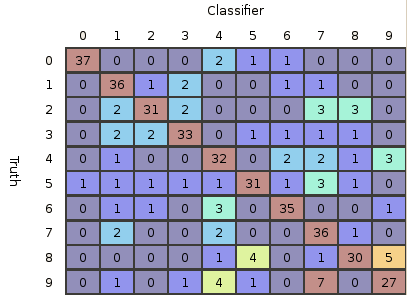
\includegraphics[width=0.9\textwidth]{images/poly_all_confusion_test.png}
\caption{Polynomial Kernel 10 Digit Test Error Confusion Matrix}
\label{poly10testconfusion}
\end{figure}

\begin{figure}
\centering
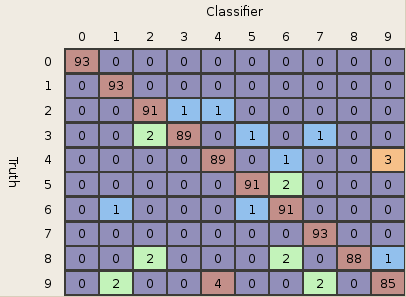
\includegraphics[width=0.9\textwidth]{images/poly_all_confusion_training.png}
\caption{Polynomial Kernel 10 Digit Training Error Confusion Matrix}
\label{poly10trainconfusion}
\end{figure}

\begin{figure}
\centering
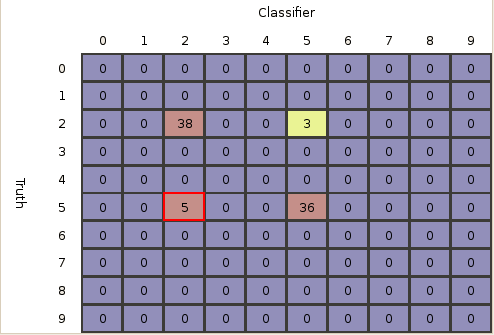
\includegraphics[width=0.9\textwidth]{images/test2_5_confusion_a0156.png}
\caption{Polynomial Kernel 2 Digit Test Error Confusion Matrix}
\label{poly2testconfusion}
\end{figure}

\begin{figure}
\centering
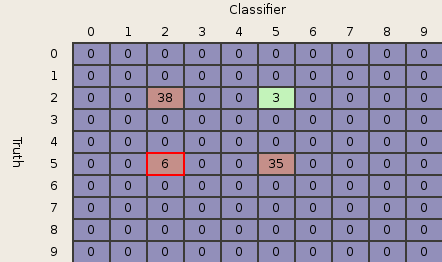
\includegraphics[width=0.9\textwidth]{images/test2_5_confusion_radial.png}
\caption{Radial Kernel 2 Digit Test Error Confusion Matrix}
\label{radial2testconfusion}
\end{figure}

\begin{figure}
\centering
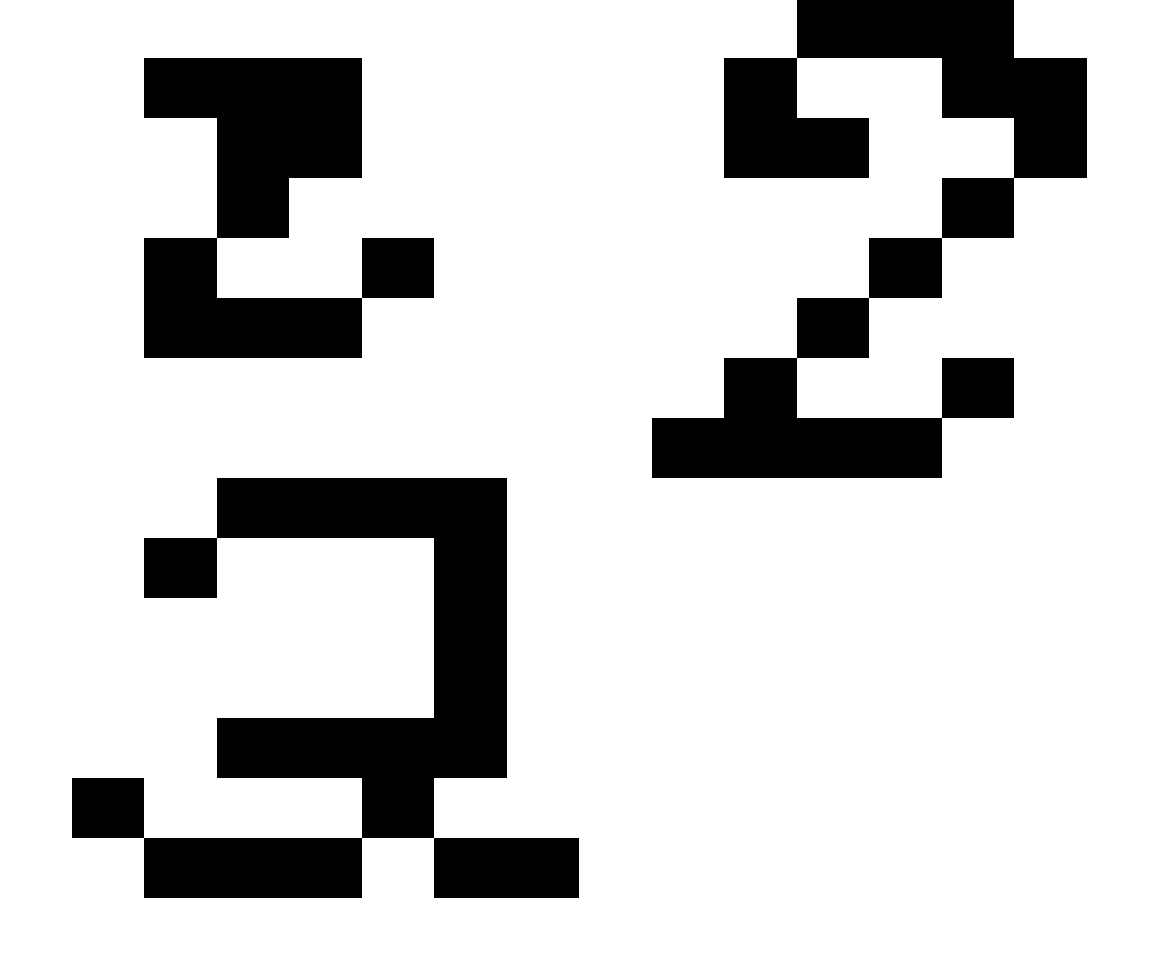
\includegraphics[width=0.9\textwidth]{images/test2_5_correct2_class5_a0156.png}
\caption{Polynomial Kernel 2 Missclassified as 5}
\label{poly2errortest}
\end{figure}

\begin{figure}
\centering
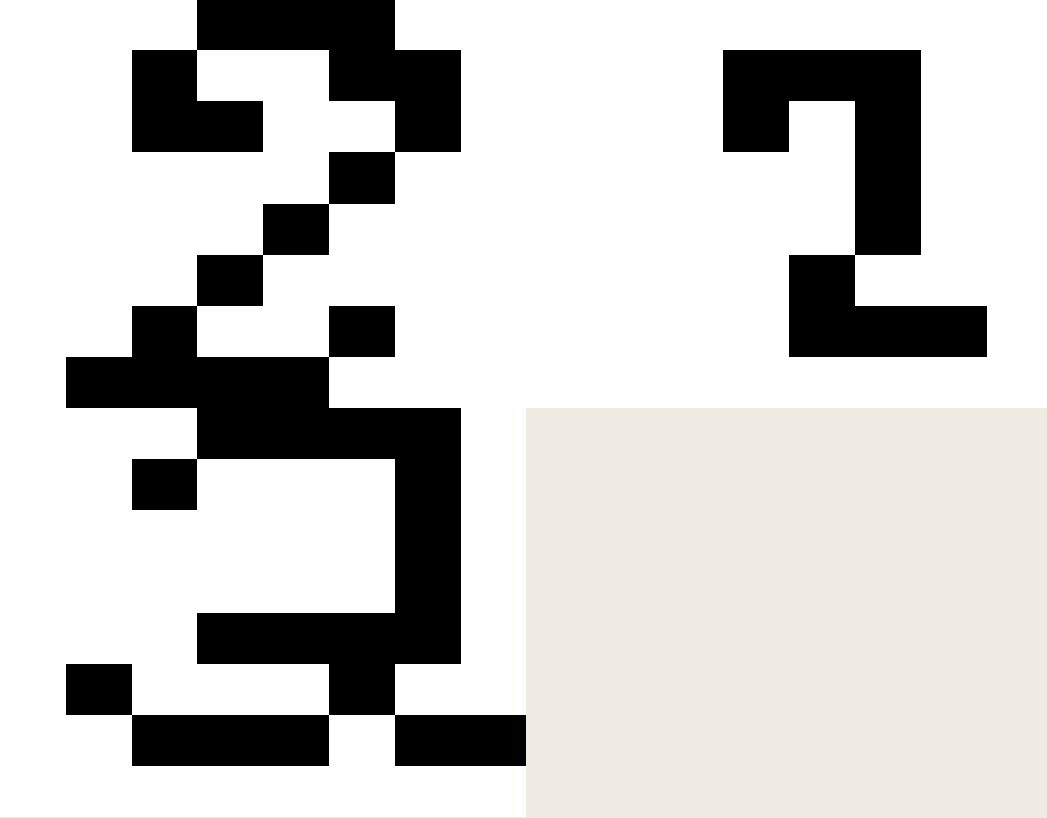
\includegraphics[width=0.9\textwidth]{images/test2_5_correct2_class5_radial.png}
\caption{Radial Kernel 2 Missclassified as 5}
\label{radial2errortest}
\end{figure}

\begin{figure}
\centering

\includegraphics[width=0.9\textwidth]{images/test2_5_correct5_class2_a0156.png}
\caption{Polynomial Kernel 5 Missclassified as 2}
\label{poly5errortest}
\end{figure}

\begin{figure}
\centering
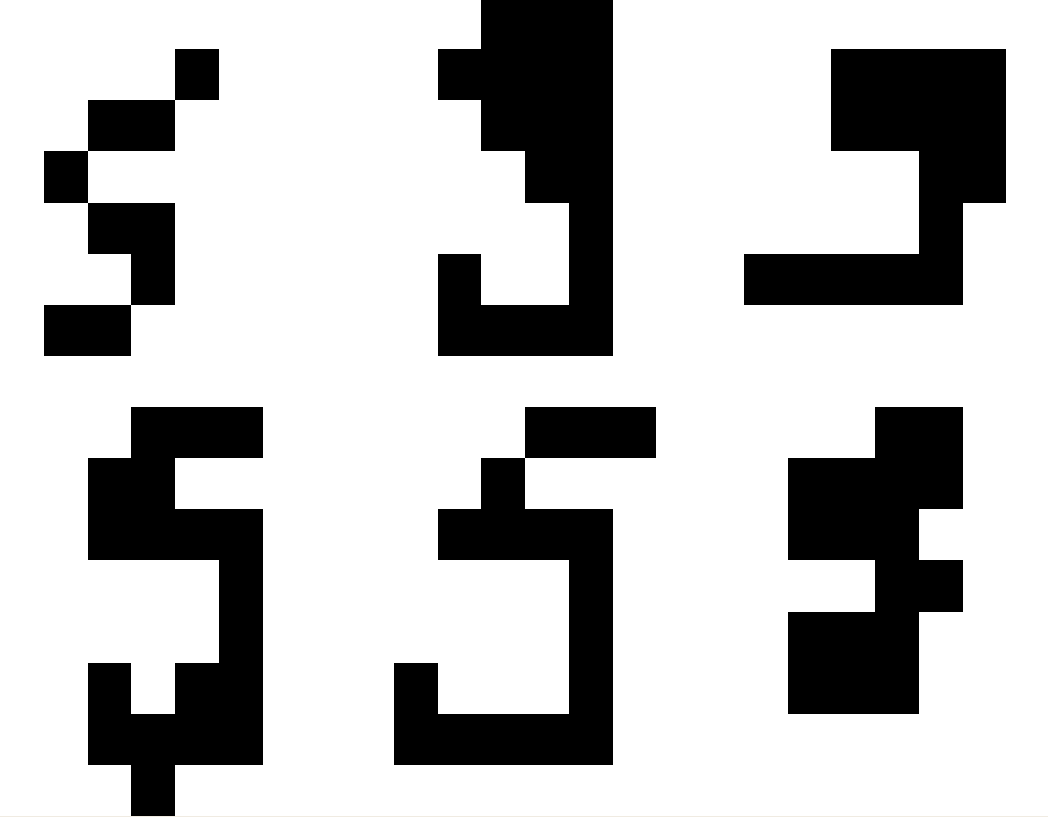
\includegraphics[width=0.9\textwidth]{images/test2_5_correct5_class2_radial.png}
\caption{Radial Kernel 5 Missclassified as 2}
\label{radial5errortest}
\end{figure}

\begin{figure}
\centering
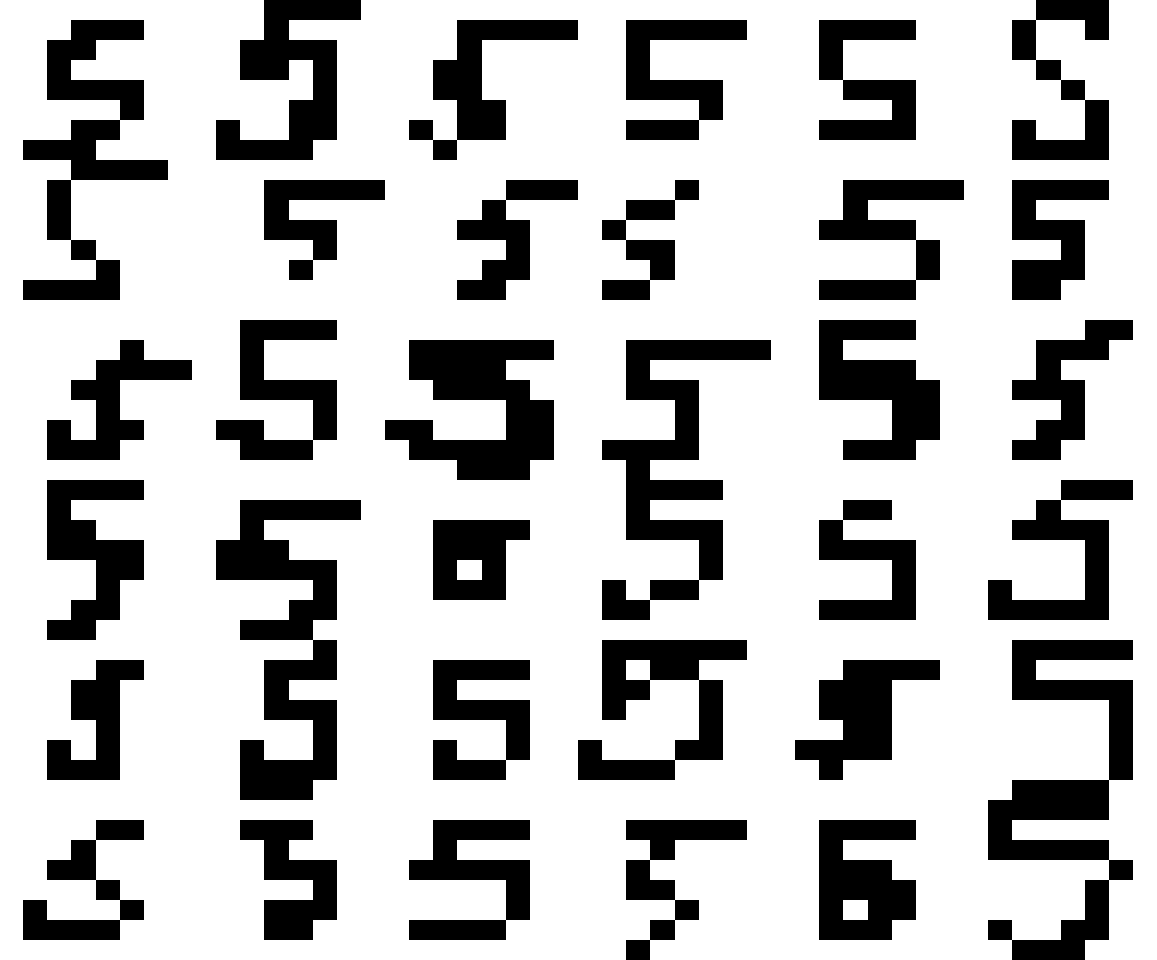
\includegraphics[width=0.9\textwidth]{images/test2_5_correct5s_a0156.png}
\caption{Polynomial Kernel Correctly Classified 5 Digits}
\label{poly5correcttest}
\end{figure}

\begin{figure}
\centering
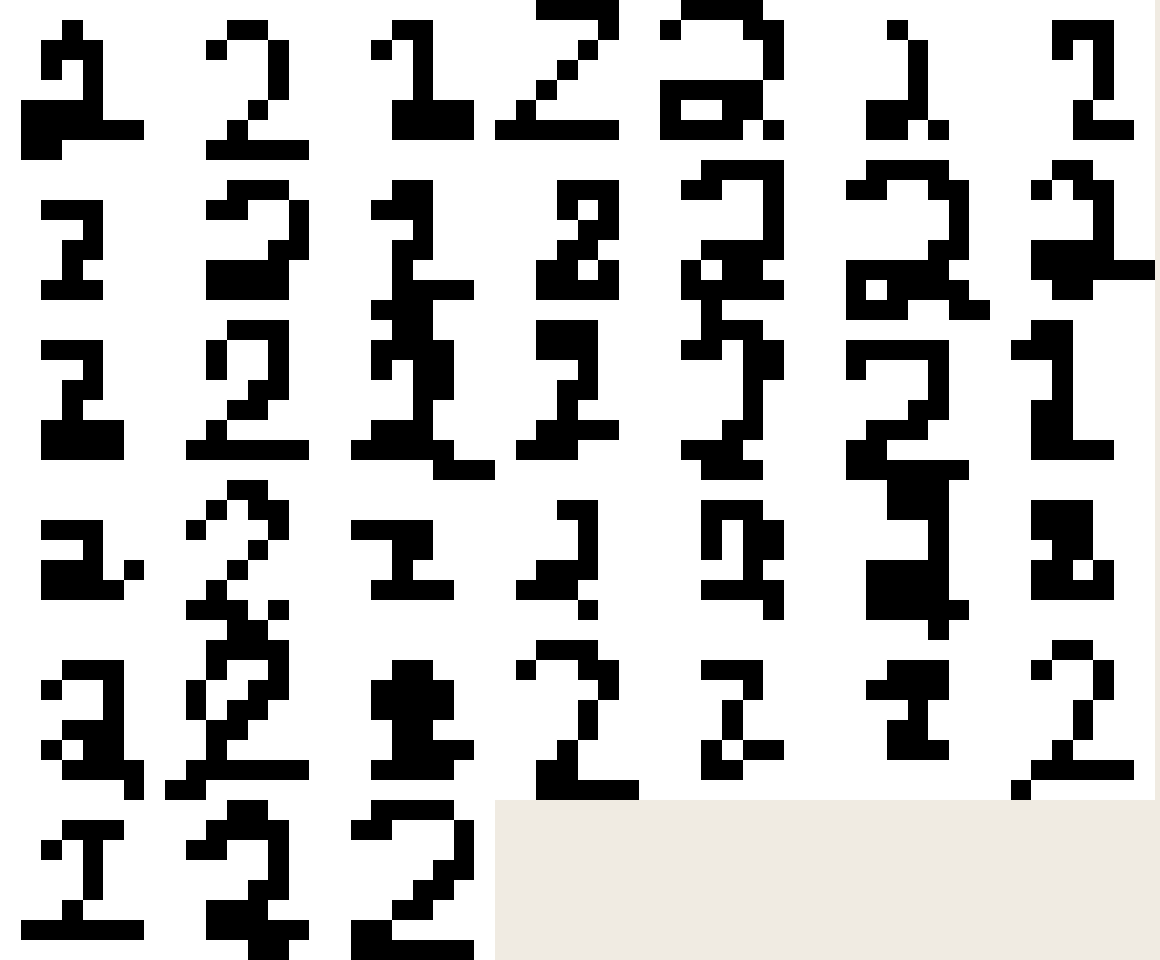
\includegraphics[width=0.9\textwidth]{images/test2_5_correct2s_a0156.png}
\caption{Polynomial Kernel Correctly Classified 2 Digits}
\label{poly2correcttest}
\end{figure}

\begin{figure}
\centering
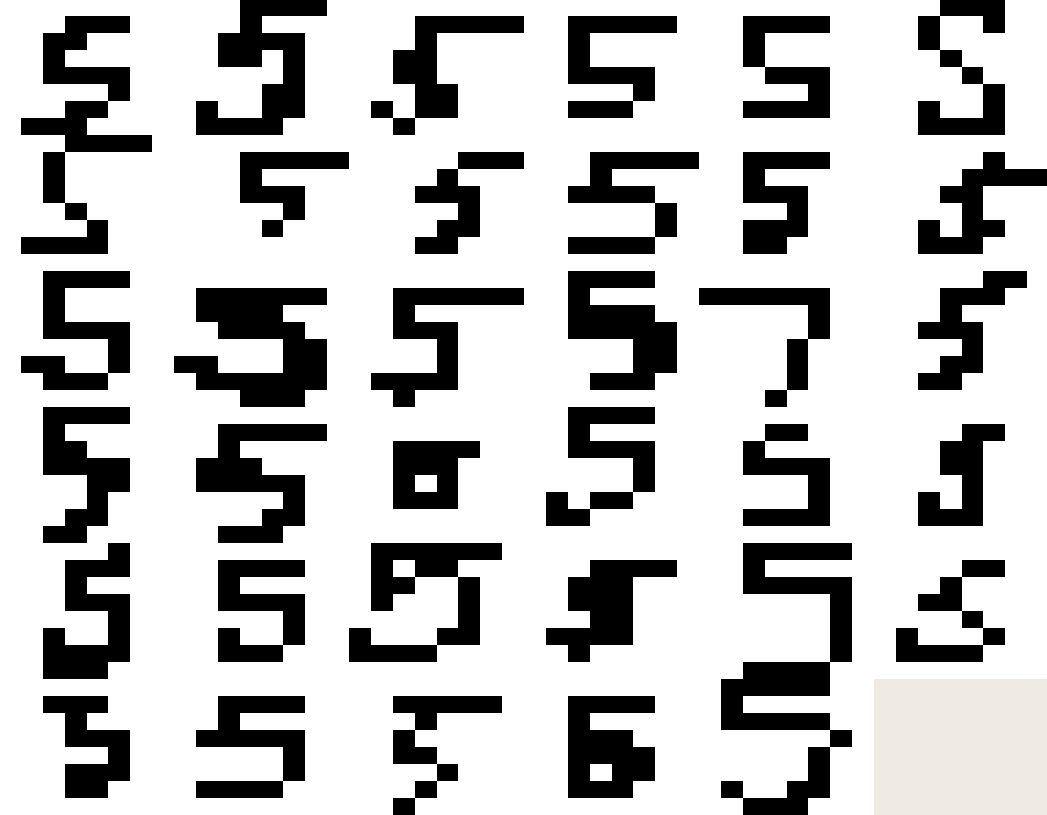
\includegraphics[width=0.9\textwidth]{images/test2_5_correct5_radial.png}
\caption{Radial Kernel Correctly Classified 5 Digits}
\label{radial5correcttest}
\end{figure}

\begin{figure}
\centering
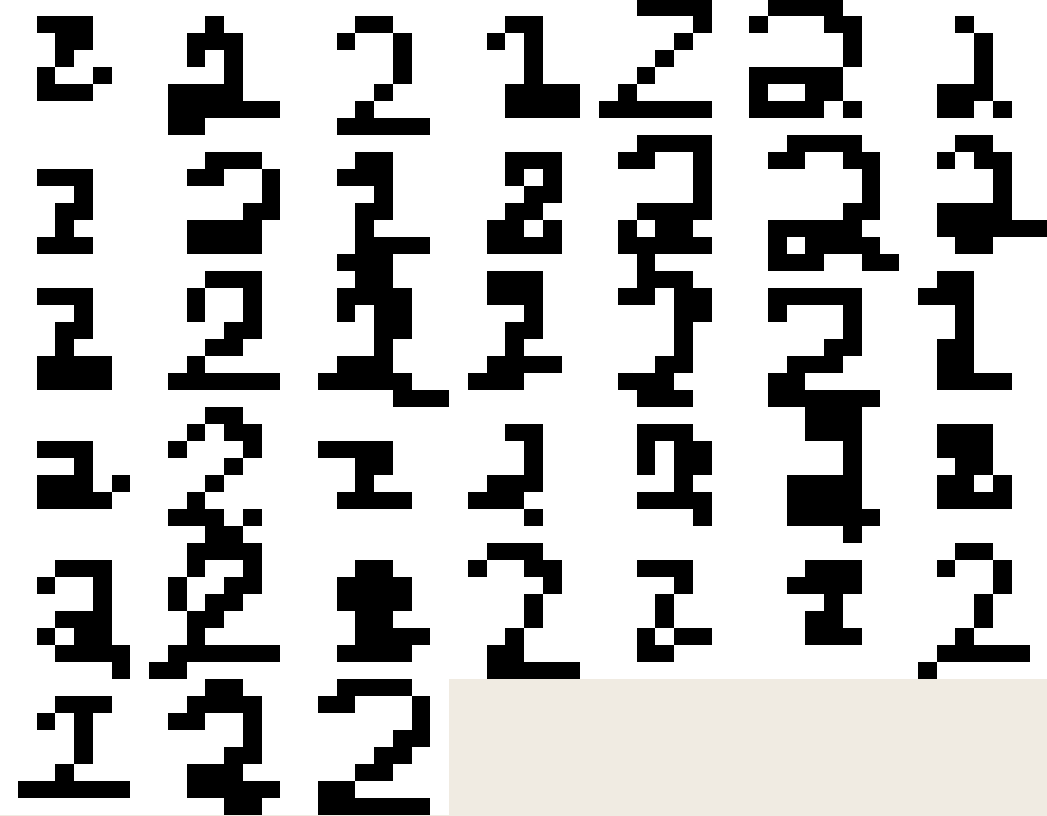
\includegraphics[width=0.9\textwidth]{images/test2_5_correct2_radial.png}
\caption{Radial Kernel Correctly Classified 2 Digits}
\label{radial2correcttest}
\end{figure}

\begin{thebibliography}{9}

\bibitem{cpl}
  Tom M. Mitchell,
  \emph{Machine Learning},
  WCB McGraw-Hill, Boston,
  1997.

\end{thebibliography}

\end{document}
